\documentclass[twocolumn]{article}
\usepackage{graphicx}
\usepackage{float}
\usepackage{stfloats}
\usepackage{hyperref}
\usepackage{lipsum}

\renewcommand{\thesection}{\Roman{section}}
\renewcommand{\thesubsection}{\Roman{section}.\Roman{subsection}}

\begin{document}

\twocolumn[{
    \begin{center}
        {\LARGE GenNarrate} \\
        \vspace{1em}
        {\large INF-3993 Generative Artificial Intelligence} \\
        \vspace{0.25em}
        {\large University of Tromsø} \\
        \vspace{1em}
        {\large Opdahl, T and Wilhelmsen, M} \\
        \vspace{0.25em}
        {\small June, 2025}
        \vspace{5em}
    \end{center}
}]

\section{Introduction}
This project explores the application of generative AI models to create an accessible, voice-driven interface for document comprehension.

This application, named \textbf{GenNarrate}, allows a user to learn about and explore a PDF document in an engaging way my being able to speak directly to an assistant that knows all about the document and is able to discuss it with a user.

The system achieves this though its retrieval-augmented generation (RAG) pipeline, which grounds the language model’s responses in relevant parts of the original document.

The goal of this project is to demonstrate how recent advancements in generative AI—specifically LLMs, TTS, and ASR—can be composed into a coherent and multimodal user experience.

\section{Technical Background}
Below we have provided a brief overview of the models and processes used in this project.

\subsection{Large Language Model (LLM)}
This project uses the DeepSeek LLM with 7B parameters\cite{deepseek7bchat}. Although small and compact in comparison to state-of-the-art LLMs, this model is still capable of advanced reasoning and language understanding. The model follows a decoder-only transformer architecture, trained using causal language modeling to predict the next token based on previous context.

In this project, the model is used to generate responses to user queries, often enhanced with additional context retrieved via a retrieval-augmented generation (RAG) pipeline. This makes it suitable for open-ended dialogue and task-oriented conversation generation, especially when combined with contextual document embeddings.

\subsection{Retrieval-Augmented Generation (RAG)}
A Retrieval-Augmented Generation (RAG) pipeline is implemented into this project to help the LLM to get valuable context to a user prompt. Given a user query, the system first encodes it using a sentence transformer model, specifically \texttt{all-MiniLM-L6-v2}\cite{allminilm2021}. It then performs a nearest-neighbor search over previously embedded documents stored in a ChromaDB vector database\cite{chromadb2023}.

The retrieved document chunks are sent along with the user prompt, allowing it to ground its generation in more accurate and domain-specific information.

\subsection{Automatic Speech Recognition (ASR)}
The model this project uses for speech recognition is Whisper from OpenAI. Whisper is a multilingual encoder-decoder transformer trained on 680,000 hours of audio data, making it robust across different languages, accents, and recording conditions\cite{radford2022whisper}. This project uses the largest variant of Whisper which is the \texttt{large-v3} variant.

Whisper processes incoming speech by first resampling it to 16kHz and then encoding the waveform before generating the corresponding text tokens. In our system, this transcribed text is passed to the language model for further processing. The use of Whisper enables hands-free interaction with the DeepSeek LLM, making the system multimodal.

\subsection{Text-to-Speech (TTS)}
To produce spoken responses, the project uses the Kokoro-82M TTS model\cite{kokoro82m}. This neural model converts generated text into speech using the \texttt{af\_heart} voice and returns an audio stream in real time.

\section{Design}
The system follows a three-tiered architecture with clearly separated frontend, backend, and inference layers. As visualized in Figure~\ref{fig:architecture}, the frontend is responsible for user interaction, the backend handles data processing and logic, and the inference engine performs the heavy computational tasks.

\begin{figure*}[htb]
    \centering
    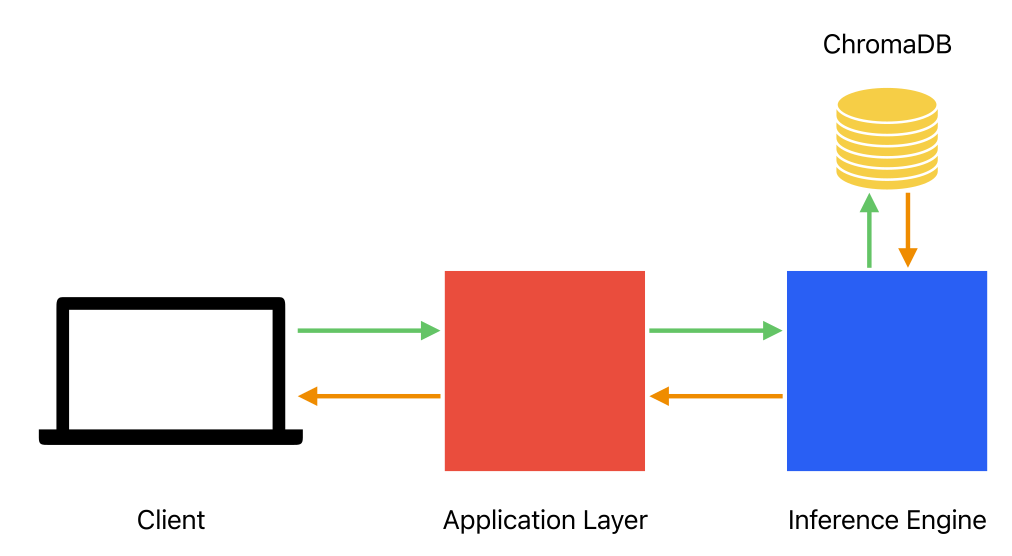
\includegraphics[width=0.75\textwidth]{imgs/architecture.png}
    \caption{System architecture of GenNarrate, illustrating the interaction between the frontend, backend, and inference engine.}
    \label{fig:architecture}
\end{figure*}

\subsection{User Interface}
The UI, also known as the frontend, is written in JavaScript with the React.js\cite{reactjs} framework. React.js is a widely adopted JavaScript library for developing user interfaces in a component-based manner. This part of the design provides a clean user-friendly experience, allowing users to interact with the system through a web browser. The UI includes features for text, voice and file input, as well as displaying the generated responses from the models.

\subsection{Application Layer}
The App Layer, also known as the backend, is written in Python using the Flask framework\cite{flaskdocs}. Flask works as an API that handles requests from the user interface and processes data logic before sent elsewhere. It pre-processes user inputs and handles CPU-intensive tasks ranging from document chunking to conversation history management. The application layer acts as a bridge between the user interface and the inference engine, ensuring no direct communication between the two.

\subsection{Inference Engine}
The inference engine, which is also a backend layer, uses the same framework as the application layer, Flask, though designed to run on separate nodes.
It is responsible for computing GPU-intensive tasks such as running the LLM, ASR, TTS, and RAG pipelines. Also hosting the ChromaDB\cite{chromadb2023} vector
database for storing and retrieving document embeddings.

\section{Implementation}
\subsection{User Interface}
The user interface consists of JavaScript functions for client-side data processing, and renders objects with HTML and CSS for styling. The JavaScript code cooperates with the HTML by using state variables to handle user actions and dynamically update the UI.

The functions for submitting audio, prompts and files share a similar structure. \\
When a user submits input to the interface, the functions appends relevant state variables to a form, and then this form is sent to the application layer through \verb|HTTP POST| requests. In the case of submitting a file of the document or audio kind, the application layer will respond with a simple success message, while a text prompt will return a full response from an AI model. These responses are added to a state variable which contains the conversation history, and is cooperating with HTML to render the conversation in a chat-like format.

However, if the user submits a text or audio prompt with the text-to-speech state variable enabled, the function will render the audio stream returned from the application layer immediately to the user interface, allowing the user to listen to the response without waiting for the full response from the AI model.

The JavaScript also enables the user to record audio using a third-party recording library.

\subsection{Application Layer}
The application layer is an API connecting the user interface to the inference engine, pre-processing data and managing conversation history. See Figure~\ref{fig:applayer} for an overview of the application layer endpoints.

\verb|/upload/speech/| serves as the endpoint for uploading audio files, and demands the audio file, \verb|history| as \verb|JSON| and the text-to-speech variable. Using a custom made function, the \verb|history| is formatted into a suitable string called \verb|conversation| for the AI models on the inference engine. The audio file is then forwarded for transcription using the \verb|/recognizeTextFromSpeech| endpoint of the inference engine. Depending on the text-to-speech variable, the response is either returned as a text string, or relayed as an audio stream to the user interface.

The \verb|/upload/text/| endpoint takes the same parameters as the previous endpoint, but instead of audio, it takes a text prompt. After processing the \verb|history| into \verb|conversation|, it forwards the prompt to the corresponding endpoint from the text-to-speech variable. If the text-to-speech variable is enabled, the request is sent to the \verb|/generateSpeechFromText| endpoint, which returns an audio stream. If the text-to-speech variable is disabled, the request is sent to the \verb|/generateTextFromText| endpoint, which returns a text response.

Out of the three, the \verb|/upload/file| endpoint handles the most intensive logic. After receiving a file, it will read the contents of the file as text, and chunk it into smaller pieces. The chunks are then sent to the \verb|/indexEmbeddings| endpoint of the inference engine which uses a sentence transformer model to return an embedding for each chunk. These embeddings are indexed using FAISS, which is a library for efficient similarity search and clustering of dense vectors. The embeddings are stored in ChromaDB\cite{chromadb2023} under a common document identifier, allowing them to be retrieved later during inference. This process enables a Retrieval-Augmented Generation (RAG) pipeline that enhances the LLM's inference capability. This endpoint returns a simple success message to the user interface, indicating that the file has been successfully processed and indexed.

\begin{figure}[H]
    \centering
    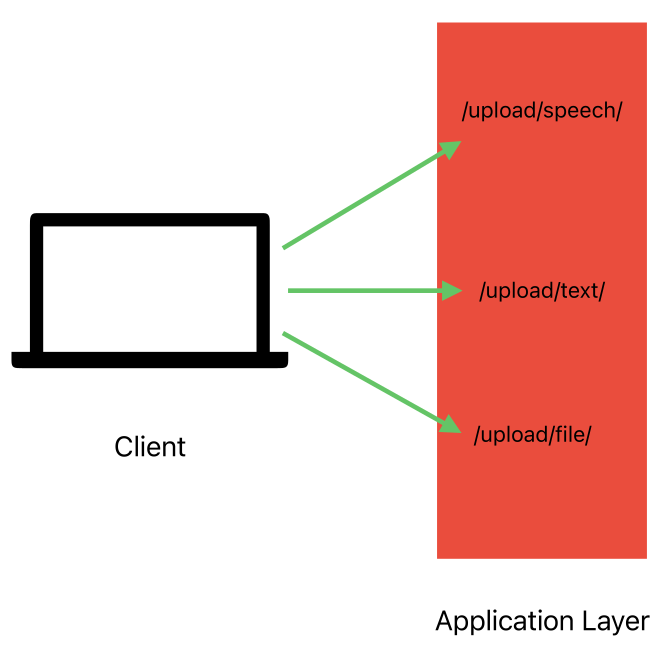
\includegraphics[width=0.75\linewidth]{imgs/applayer.png}
    \caption{Overview of the application layer endpoints}
    \label{fig:applayer}
\end{figure}

\subsection{Inference Engine}
For this section, we will emphasize the models in order to reflect the course content. See Figure~\ref{fig:inference} for an overview of the inference engine and its connection to the application layer and the database.

\subsubsection{DeepSeek LLM}
The inference engine loads the\\\texttt{deepseek-llm-7b-chat}\cite{deepseek7bchat} model using the Hugging Face \texttt{transformers} library. Its initialized with \texttt{float16} precision and moved to GPU memory on server startup for better efficiency. To avoid unessecary gradient computations, the model is paired with a corresponding tokenizer which is set to evaluation mode.\\
Each incoming request includes the conversation history and current prompt. Before generation, the system retrieves contextual information from ChromaDB. The context is always added to the prompt string if context is available. The fully assembled query is then tokenized and passed to the model, the generatd output is then decoded and returned as text.

\subsubsection{RAG with Chroma DB}
\begin{figure*}[htb]
    \centering
    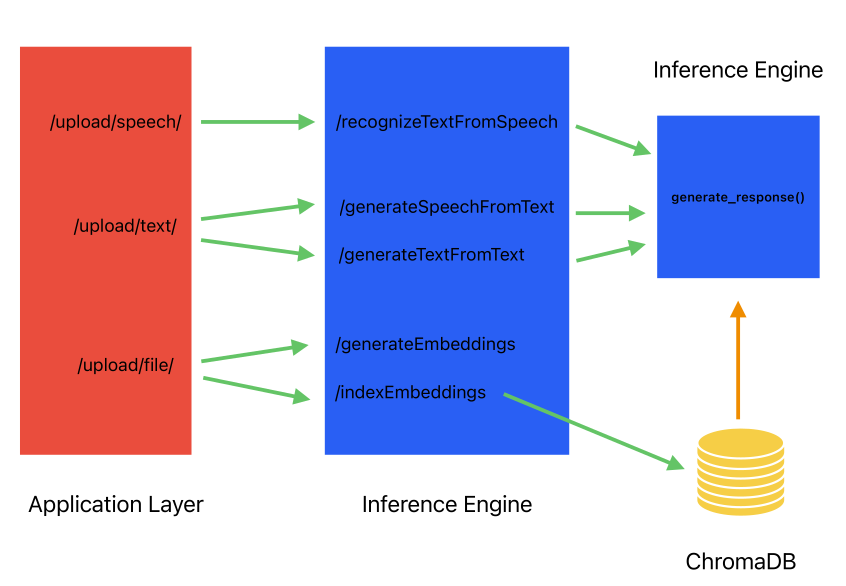
\includegraphics[width=0.75\textwidth]{imgs/inference.png}
    \caption{Overview of the inference engine and connection to the application layer}
    \label{fig:inference}
\end{figure*}

The Retrieval-Augmented Generation (RAG) component uses the \texttt{all-MiniLM-L6-v2} model from SentenceTransformers to embed both user prompts and document chunks. On startup, the embedding model is loaded onto the GPU.

Document chunks are embedded and stored using ChromaDB\cite{chromadb2023}, a persistent vector database. When a user prompt is received, it is embedded and used to query ChromaDB for the top-k most relevant chunks. These chunks are spliced together into a single context string and added to the context of the LLM input.\\
There are two endpoints in the inference engine that facilitates for storing files in the Chroma DB.
\begin{itemize}
    \item \textbf{/generateEmbeddings:} endpoint receives raw text chunks and returns their vector embeddings using the MiniLM model.
    \item \textbf{/indexEmbeddings:} endpoint receives both the raw chunks and their precomputed embeddings, and stores them in ChromaDB under a common document identifier. Each chunk is assigned a unique ID to support retrieval later during inference.
\end{itemize}

\subsection{ASR with Whisper}
The Automatic Speech Recognition (ASR) component uses OpenAI’s \texttt{whisper-large-v3}\cite{radford2022whisper} model to transcribe user audio input into text. The model is loaded onto the GPU at server startup and used through a Hugging Face pipeline for streamlined inference.

Incoming audio is received as a file upload and is then loaded into memory using \texttt{torchaudio}\cite{torchaudio}. Since most microphones use 44.1kHz or 48kHz, all audio is resamples to meet Whisper's requirement of 16kHz before inference. If the audio is stereo, it is down-mixed to mono. When the transcription is complete, the resulting text is then appended to the conversation history and passed on for further response generation for the LLM.

This component powers hands-free interaction via the \texttt{/recognizeTextFromSpeech} endpoint and enables the system to support voice-based dialogue.

\subsubsection{TTS with Kokoro}
The Text-to-Speech (TTS) component uses the Kokoro-82M model\cite{kokoro82m} to synthesize audio from text. The model is accessed through the \texttt{KPipeline} interface, which produces audio in small chunks suitable for streaming.

Audio chunks are streamed as they are created using Flask's \texttt{stream\_with\_context} and encoded as WAV using the \texttt{soundfile}\cite{soundfile} library. Doing this makes it so the system delivered speech responses with minimal delay.

\subsubsection{Endpoints Overview}
\begin{itemize}
    \item \textbf{/recognizeTextFromSpeech:} Generates text audio sent by user to then pass on for further processing by the \texttt{generate\_response()} function (see Section \ref{sec:functions}).
    \item \textbf{/generateTextFromText:} Endpoint that\\ receives prompt from user, and sends prompt on for further processing with the \texttt{generate\_response()} function before feeding to the LLM.
    \item \textbf{/generateSpeechFromText:} Receives user prompt, processes full query and receives respons from LLM, then sends audio stream back with function \texttt{generate\_audio\_stream()} that creates audio from the text provided by the LLM.
\end{itemize}

\subsubsection{Importiant Functions}
\label{sec:functions}
\begin{itemize}
    \item \textbf{generate\_response(conversation, prompt):} This function handles the end-to-end logic for generating a text response to a user prompt. First, the prompt is embedded and used to query ChromaDB for relevant document chunks, forming a contextual grounding string. The prompt is then classified via a zero-shot classifier to determine intent.

    Based on the classification, the function selects the appropriate model and tokenizer (currently only the DeepSeek LLM is used). The conversation history and context are formatted into a full prompt and passed to the model for generation. The output is cleaned and returned as a plain string.
    \item \textbf{generate\_audio\_stream(text):} This function uses the Kokoror TTS pipeline to transform input text into speech. The Kokoro pipeline returns an iterator over audio chunks, which are encoded into WAV format. The function yields these chunks incrementally via a Flask stream, enabling real-time audio playback in the client.
\end{itemize}

\section{Experiments and Results}
To evaluate the performance of the inference engine, we conducted a series of timing experiments focused on the language model component. The goal was to assess how the system scales with different levels of input and output complexity. In each experiment, the prompt was varied in length and expected output size, while all other conditions remained constant. Each prompt configuration was tested five times to account for natural variation in inference time.

The server was restarted between experiments to ensure consistent baseline conditions with no prior conversation history.

\subsection{Prompt Categories}
We defined four prompt categories:
\begin{itemize}
    \item \textbf{Short prompt, short output:} A single-sentence query expecting a brief response.
    \item \textbf{Medium prompt, medium output:} Two-sentence input with a more informative paragraph-length response.
    \item \textbf{Long prompt, long output:} Three-sentence query requiring a multi-paragraph answer.
    \item \textbf{Extended prompt, extended output:} A detailed four-sentence prompt with an expected response of over 700 tokens.
\end{itemize}

\subsection{LLM Inference Time}
The timing results for each prompt category are summarized in Figure~\ref{fig:inference-times}. Each bar represents the average inference time for that category, with error bars showing standard deviation across the five runs.
\begin{figure}[H]
    \centering
    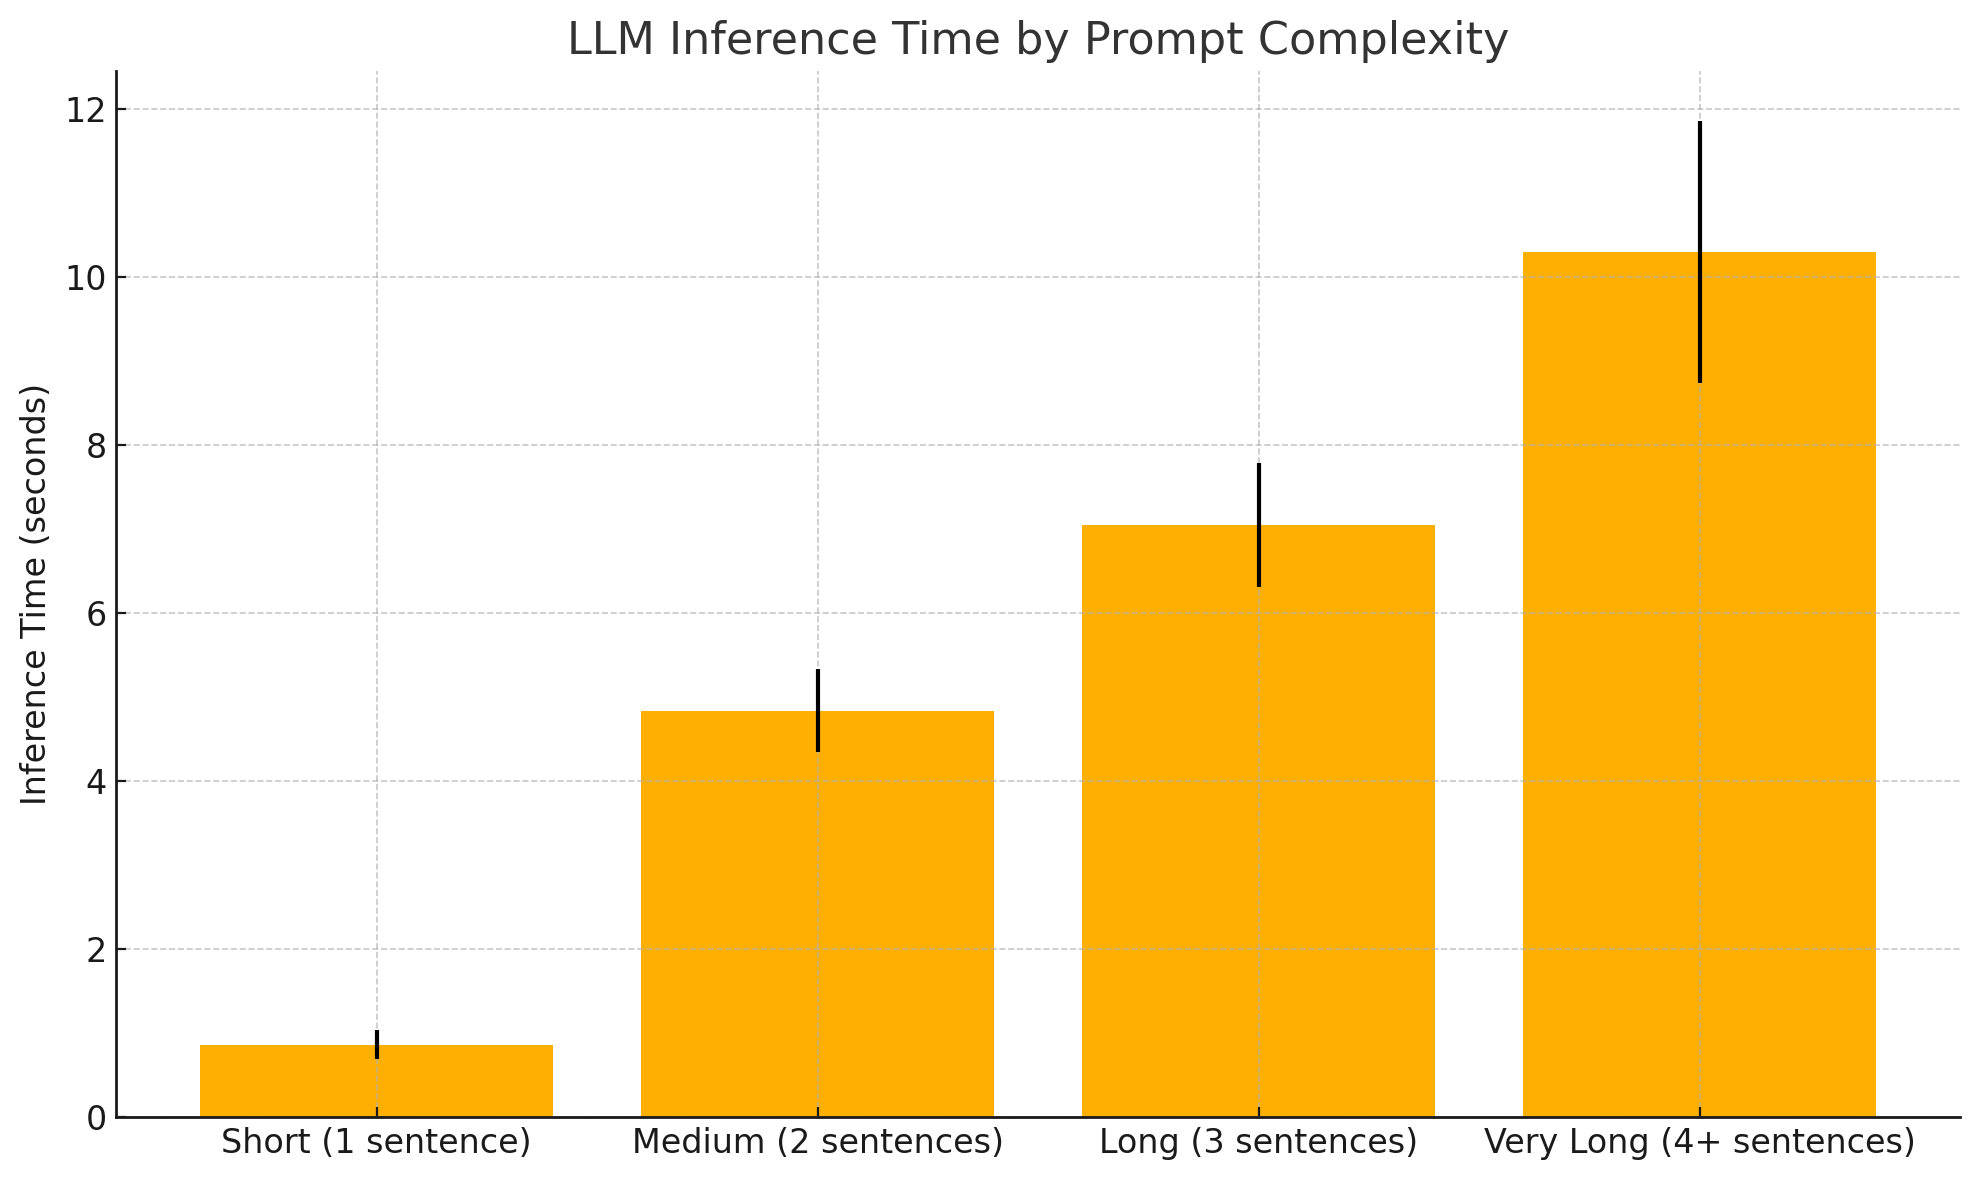
\includegraphics[width=\linewidth]{imgs/output.png} 
    \caption{Average LLM inference time for prompts of increasing complexity.}
    \label{fig:inference-times}
\end{figure}
The results show a clear upward trend in inference time as prompt and output complexity increases. The shortest queries averaged under one second, while the most demanding prompt required over 10 seconds on average. This demonstrates how prompt design can significantly influence response latency, which is an important consideration in real-time or user-facing applications.

\subsection{Other Tests}
Additional tests where also conducted to check the functionality and user-friendliness of the application, to give us an idea on further improvements and see that what implemented actually works the way it should work. Since this is not measurable by any meaningful metrics, this report will not cover this as it would not be scientific.

Although we will not include these tests in detail, the tests we have done to test overall system functionality has been successful.

\section{Discussion}
\subsection{Unfinished Features}
In the implementation of the backend server, there is a implementation of a feature that is not yet finished as it does not communicate with the frontend. The features goal is to take a PDF file, and send this file to a GPT-4 model using OpenAI's API, so that this model can separate the PDF into narratable chunks that are contextually made, meaning that the document is split up in such a way that there is natural pauses between each chunk, so that each chunk stops at an appropriate point in the text and is not awkward, enhancing user experienceS.

This enables the user to have the application read the document to them, chunk by chunk, so that the user can ask questions about the chunk they just heard. 

The reason for choosing to go for a larger LLM in this case is simple, its a different way of interacting with a LLM, and also the model on the inference server cannot handle very large documents, something GPT4 handles exceptionally better.

\section{Conclusion}
GenNarrate demonstrates how generative AI models can be combined to form an end-to-end multimodal system for document comprehension. By integrating a large language model, a TTS engine, and optional ASR functionality, the system allows users to consume and interact with written documents through speech.

The architecture was designed with clarity and modularity in mind, separating the inference engine from the application logic and user interface.

Although this project is built for a single-user research setting, it showcases the potential of deploying conversational AI beyond traditional chat interfaces.

\subsubsection{}
\bibliographystyle{plain}
\bibliography{ref}
\end{document}
